\documentclass{article}
\usepackage[utf8]{inputenc}
\usepackage{verbatim}
\usepackage{amsmath}
\usepackage{enumerate}
\usepackage{amsfonts}
\usepackage{microtype}
\usepackage{todonotes}
\usepackage[english]{babel}
\usepackage{graphicx}
\usepackage{tikz}
\usepackage[bottom]{footmisc}

\def\checkmark{\tikz\fill[scale=0.4](0,.35) -- (.25,0) -- (1,.7) -- (.25,.15) -- cycle;}

\title{dRegAut afl 4}
\author{Hanus Rindom}
\date{May 2014}

\begin{document}

\maketitle

\section*{Martin, opg. 2.55 (c)}
The first thing the algortihm does is to eliminate states not connedtet with the initial state, this will not change the language accepete by the FA.\\
This being done we can assume all states of the FA is reachable form the initial state 1.\\
The first thing the minimization algorithm looks for is distingseble states , such as an accepting state with an nonaccepting state.\\

Now we go through every pair, testing, and comparing, creating an table:

\begin{table}[h]
\begin{tabular}{ccccccc}
\cline{2-2}
\multicolumn{1}{l|}{2} & \multicolumn{1}{l|}{3} &                        &                        &                        &                        &                       \\ \cline{2-3}
\multicolumn{1}{l|}{3} & \multicolumn{1}{l|}{2} & \multicolumn{1}{l|}{2} &                        &                        &                        &                       \\ \cline{2-4}
\multicolumn{1}{l|}{4} & \multicolumn{1}{l|}{2} & \multicolumn{1}{l|}{2} & \multicolumn{1}{l|}{2} &                        &                        &                       \\ \cline{2-5}
\multicolumn{1}{l|}{5} & \multicolumn{1}{l|}{2} & \multicolumn{1}{l|}{2} & \multicolumn{1}{l|}{2} & \multicolumn{1}{l|}{\checkmark}  &                        &                       \\ \cline{2-6}
\multicolumn{1}{l|}{6} & \multicolumn{1}{l|}{1} & \multicolumn{1}{l|}{1} & \multicolumn{1}{l|}{1} & \multicolumn{1}{l|}{1} & \multicolumn{1}{l|}{1} &                       \\ \cline{2-7} 
\multicolumn{1}{l|}{7} & \multicolumn{1}{l|}{1} & \multicolumn{1}{l|}{1} & \multicolumn{1}{l|}{1} & \multicolumn{1}{l|}{1} & \multicolumn{1}{l|}{1} & \multicolumn{1}{l|}{\checkmark} \\ \cline{2-7} 
                       & 1                      & 2                      & 3                      & 4                      & 5                      & 6                    
\end{tabular}
\end{table}


Pairs marked 1 are the accepting states, these are found on the first pass.\\
Pairs marked 2 and 3 are marked on the second and third pass. As we can see only pair $ \{ 1,2 \} $ is marked with 3. Which is because it is consideret after pair $ \{ 1,3 \} $, and will have to wait for the third pass. \\
The algorithm ran through the table vertical, filling the two first lines with 1\footnote{except $ \{ 7,6 \} $ since they both are acceptingstates}.\\

Two boxes in the table is marked with an checkmarks, these is the accepted pairs. These we can combine to form the minimized FA.
\begin{center}
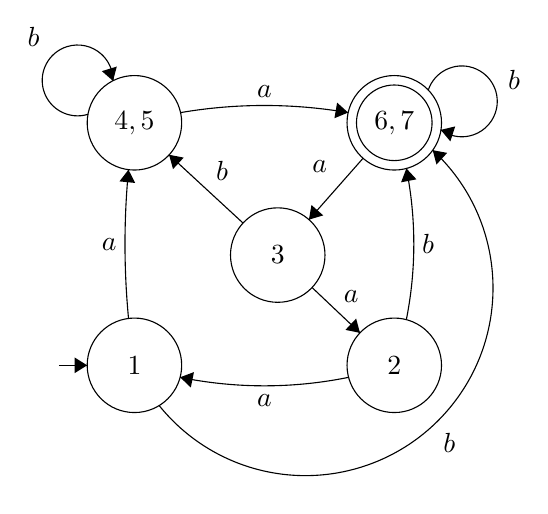
\begin{tikzpicture}[scale=0.2]
\tikzstyle{every node}+=[inner sep=0pt]
\draw [black] (8.3,-22) circle (3);
\draw (8.3,-22) node {$1$};
\draw [black] (24.8,-22) circle (3);
\draw (24.8,-22) node {$2$};
\draw [black] (17.4,-15) circle (3);
\draw (17.4,-15) node {$3$};
\draw [black] (8.3,-6.6) circle (3);
\draw (8.3,-6.6) node {$4,5$};
\draw [black] (24.8,-6.6) circle (3);
\draw (24.8,-6.6) node {$6,7$};
\draw [black] (24.8,-6.6) circle (2.4);
\draw [black] (3.5,-22) -- (5.3,-22);
\fill [black] (5.3,-22) -- (4.5,-21.5) -- (4.5,-22.5);
\draw [black] (7.925,-19.024) arc (-174.54658:-185.45342:49.707);
\fill [black] (7.92,-9.58) -- (7.35,-10.32) -- (8.35,-10.42);
\draw (7.2,-14.3) node [left] {$a$};
\draw [black] (27.236,-8.337) arc (47.2947:-141.24457:11.914);
\fill [black] (27.24,-8.34) -- (27.48,-9.25) -- (28.16,-8.51);
\draw (28.3,-26.29) node [below] {$b$};
\draw [black] (21.9,-22.763) arc (-78.47578:-101.52422:26.78);
\fill [black] (11.2,-22.76) -- (11.88,-23.41) -- (12.08,-22.43);
\draw (16.55,-23.8) node [below] {$a$};
\draw [black] (25.566,-9.499) arc (11.29795:-11.29795:24.508);
\fill [black] (25.57,-9.5) -- (25.23,-10.38) -- (26.21,-10.19);
\draw (26.54,-14.3) node [right] {$b$};
\draw [black] (19.58,-17.06) -- (22.62,-19.94);
\fill [black] (22.62,-19.94) -- (22.38,-19.03) -- (21.7,-19.75);
\draw (22.07,-18.02) node [above] {$a$};
\draw [black] (15.2,-12.97) -- (10.5,-8.63);
\fill [black] (10.5,-8.63) -- (10.75,-9.54) -- (11.43,-8.81);
\draw (13.87,-10.31) node [above] {$b$};
\draw [black] (5.361,-6.058) arc (287.27298:-0.72702:2.25);
\draw (2.31,-1.17) node [left] {$b$};
\fill [black] (6.94,-3.94) -- (7.18,-3.03) -- (6.23,-3.32);
\draw [black] (11.228,-5.953) arc (99.73038:80.26962:31.488);
\fill [black] (21.87,-5.95) -- (21.17,-5.32) -- (21,-6.31);
\draw (16.55,-5) node [above] {$a$};
\draw [black] (22.82,-8.85) -- (19.38,-12.75);
\fill [black] (19.38,-12.75) -- (20.29,-12.48) -- (19.54,-11.82);
\draw (20.56,-9.35) node [left] {$a$};
\draw [black] (26.955,-4.529) arc (161.59605:-126.40395:2.25);
\draw (32,-3.9) node [right] {$b$};
\fill [black] (27.75,-7.05) -- (28.36,-7.78) -- (28.67,-6.83);
\end{tikzpicture}
\end{center}

\end{document}
